\documentclass{article}
\usepackage[utf8]{inputenc}
\usepackage{amsmath}
\usepackage{mathtools}
\usepackage{tcolorbox}
\usepackage{float}
\usepackage{amsfonts}
\usepackage{svg}
\date{}

\title{\textbf{Quantum Computing: An Applied Approach}\\\vspace*{1cm}
Chapter 3 Problems: \\
Qubits, Operators and Measurement
}

\begin{document}

\maketitle

\section{}

\subsection*{(a)}

\begin{figure}[H]
  \centering
  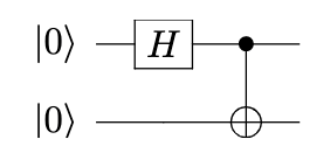
\includegraphics[width=0.4 \linewidth]{images/circuit_diagram_1.png}
\end{figure}

Qubit states transform as $|00\rangle\rightarrow\frac{|00\rangle+|11\rangle}{\sqrt{2}}\rightarrow\boxed{\frac{|00\rangle+|11\rangle}{\sqrt{2}}}$

\subsection*{(b)}

\begin{figure}[H]
  \centering
  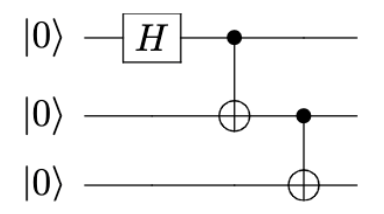
\includegraphics[width=0.4 \linewidth]{images/circuit_diagram_2.png}
\end{figure}

Qubit states transform as $|000\rangle\rightarrow
\frac{|000\rangle+|100\rangle}{\sqrt{2}}\rightarrow
\frac{|000\rangle+|110\rangle}{\sqrt{2}}\rightarrow
\boxed{\frac{|000\rangle+|111\rangle}{\sqrt{2}}}$

\subsection*{(c)}

\begin{figure}[H]
  \centering
  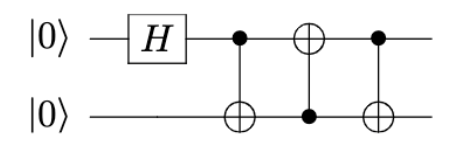
\includegraphics[width=0.4 \linewidth]{images/circuit_diagram_3.png}
\end{figure}

Qubit states transform as $|00\rangle\rightarrow
\frac{|00\rangle+|10\rangle}{\sqrt{2}}\rightarrow
\frac{|00\rangle+|11\rangle}{\sqrt{2}}\rightarrow
\frac{|00\rangle+|01\rangle}{\sqrt{2}}
\rightarrow
\boxed{\frac{|00\rangle+|01\rangle}{\sqrt{2}}}$

\section{}

\subsection*{(a)}

$|0\rangle\sim\boxed{(0,0,1)}$

\subsection*{(b)}

$|0\rangle\sim\boxed{(0,0,-1)}$

\subsection*{(c)}

$
\frac{|0\rangle+|1\rangle}{\sqrt{2}}\sim\boxed{(1,0,0)}$

\subsection*{(d)}

$
\frac{|0\rangle+e^{i\phi}|1\rangle}{\sqrt{2}}\sim\boxed{(cos(\phi),sin(\phi),0)}$

For the given parameterizations of $\phi$:

\begin{flalign*}
&\phi=0: \boxed{(1,0,0)} &\\
&\phi=\frac{\pi}{2}: \boxed{(0,1,0)} &\\
&\phi=\pi: \boxed{(-1,0,0)} &\\
&\phi=\frac{3\pi}{2}: \boxed{(0,-1,0)} &\\
\end{flalign*}

\subsection*{(e)}

$
\frac{3}{5}|0\rangle+\frac{4}{5}|1\rangle\sim \boxed{(0.96,0,-0.28)}$\\

\textbf{Note}:\\
The general expression for a pure qubit state is $|\psi\rangle=cos(\frac{\theta}{2})+e^{i\phi}sin(\frac{\theta}{2})|1\rangle$, while the corresponding qubit state can be represented by the point on the point $(sin(\theta)cos(\phi),sin(\theta)sin(\phi),cos(\theta))$ on the Bloch sphere. For a given qubit state of the form $|\psi\rangle=a|0\rangle+b|1\rangle$ with $a,b\in\mathbb{C}$, the angle $\theta$ satisfies $\theta=2\text{Arctan}(\frac{a}{b})$ while $\phi=Arg(b)$.

For the state $\frac{3}{5}|0\rangle+\frac{4}{5}|1\rangle$,  $\theta=2\text{Arctan}(\frac{3}{4})=1.855$ radians and $\phi=0$ so that $(x,y,z)=(0.96,0,-0.28)$.

\section{}

\subsection*{(a)}

The state $\frac{3}{5}|0\rangle+\frac{4}{5}|1\rangle$ lies in the xz-plane, so it can be reached by rotating an initialized $|0\rangle$ state about the y-axis.

As calculated in part 2(e), this corresponds to a rotation angle $\theta=0.59\pi$ so that this circuit can be modeled as:

\begin{figure}[H]
  \centering
  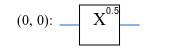
\includegraphics[width=0.4\linewidth]
  {images/circuit_a.png}
\end{figure}

\subsection*{(b)}

The state $\frac{|0\rangle+e^{i\phi}|1\rangle}{\sqrt{2}}$ where $\phi\in\{0,\frac{\pi}{2},\pi,\frac{3\pi}{2}\}$ lies on the equator of the Bloch sphere, at a rotation of $\phi$ radians about the z-axis. To form this state from an initialization of a qubit in the $|0\rangle$ state, rotate the $|0\rangle$ state onto the equator using a square root-Y gate, staying in the xz-plane, then perform an additional azimuthal rotation in increments of $\frac{\pi}{2}$ using successive S gates:

\begin{figure}[H]
  \centering
  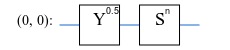
\includegraphics[width=0.4\linewidth]
  {images/circuit_b.png}
\end{figure}

where $n=\frac{2\phi}{\pi}$.

\section{}

\subsection*{(a)}

No, this is a subset of the Clifford group of operators that, by the Gottesman-Knill Theorem, generates only the set of quantum algorithms efficiently simulatable on a classic computer.

\subsection*{(b)}

No, this is equivalent to the generators of the Clifford group.

\subsection*{(c)}

Yes, this is a superset of the universal gate set \{CNOT,T,H\}.

\subsection*{(d)}

Yes, this is equal to the universal gate set \{CNOT,T,H\}.

\subsection*{(e)}

No, the CZ gate just swaps between basis elements and $H$ and $S$ are generators of the Clifford group. In fact, the CZ gate can be formed by inserting a Hadamard gate before and after the X operation on the target qubit line. This gate set can then be generated by the Clifford  group.

\subsection*{(f)}

This gate set is universal, as a CNOT can likewise be formed from a CZ gate by inserting a Hadamard before and after the X gate on the target line. The universal generating set \{CNOT,T,H\} can then be formed from these gates, from which any unitary can be generated.

\subsection*{(g)}

Yes, CNOT gates with arbitrary single-qubit unitary rotations form a universal gate set.

\subsection*{(h)}

Yes; the Hadamard is included in the set of unitary single-qubit rotations, and when placed before and after the $Z$ gate in the target line of the CZ can form a CNOT gate. Then the set \{CNOT, U\} generates \{CZ, U\} so that this gate set is also universal.

\section{}

Let $\sigma\in\{X,Y,Z\}$.
$$e^{i\theta\sigma}=\sum_{n=0}^{\infty}\frac{(i\theta\sigma)^n}{n!}$$
$$=\sum_{n=0}^{\infty}\frac{(-1)^n(\theta\sigma)^{2n}}{(2n)!}+\sum_{n=0}^{\infty}\frac{(-1)^n(\theta\sigma)^{2n+1}}{(2n+1)!}$$
$$=\sum_{n=0}^{\infty}\frac{(-1)^n(\theta)^{2n}}{(2n)!}I+i\sum_{n=0}^{\infty}\frac{(-1)^n(\theta)^{2n+1}\sigma}{(2n+1)!}\textnormal{ (by the property }\sigma^2=I)=$$
$$
\boxed{cos(\theta)I+i\textnormal{sin}(\theta)\sigma}
$$

\section{}

$$R_x(\theta)\coloneqq e^{\frac{i\theta X}{2}}=\textnormal{cos}(\frac{\theta}{2})I+i\textnormal{sin}(\frac{\theta}{2})X=
\begin{pmatrix}
\textnormal{cos}(\frac{\theta}{2}) & i\textnormal{sin}(\frac{\theta}{2})\\
i\textnormal{sin}(\frac{\theta}{2}) & \textnormal{cos}(\frac{\theta}{2})
\end{pmatrix}$$

$$R_y(\theta)\coloneqq e^{\frac{i\theta Y}{2}}=\textnormal{cos}(\frac{\theta}{2})I+i\textnormal{sin}(\frac{\theta}{2})Y=
\begin{pmatrix}
\textnormal{cos}(\frac{\theta}{2}) & \textnormal{sin}(\frac{\theta}{2})\\
-\textnormal{sin}(\frac{\theta}{2}) & \textnormal{cos}(\frac{\theta}{2})
\end{pmatrix}$$

$$R_z(\theta)\coloneqq e^{\frac{i\theta Z}{2}}=\textnormal{cos}(\frac{\theta}{2})I+i\textnormal{sin}(\frac{\theta}{2})Z=
\begin{pmatrix}
\textnormal{cos}(\frac{\theta}{2}) + i\textnormal{sin}(\frac{\theta}{2}) & 0\\
0 & \textnormal{cos}(\frac{\theta}{2}) - i\textnormal{sin}(\frac{\theta}{2})
\end{pmatrix}$$

\section{}

\subsection*{(a)}

$$R_x(\theta_2)R_x(\theta_1)=
\begin{pmatrix}
\textnormal{cos}(\frac{\theta_2}{2}) & i\textnormal{sin}(\frac{\theta_2}{2})\\
i\textnormal{sin}(\frac{\theta_2}{2}) & \textnormal{cos}(\frac{\theta_2}{2})
\end{pmatrix}\cdot
\begin{pmatrix}
\textnormal{cos}(\frac{\theta_1}{2}) & i\textnormal{sin}(\frac{\theta_1}{2})\\
i\textnormal{sin}(\frac{\theta_1}{2}) & \textnormal{cos}(\frac{\theta_1}{2})
\end{pmatrix}=
$$
$$
\begin{pmatrix}
\textnormal{cos}(\frac{\theta_2}{2})\textnormal{cos}(\frac{\theta_1}{2}) - \textnormal{sin}(\frac{\theta_2}{2})\textnormal{sin}(\frac{\theta_1}{2}) & i[\textnormal{cos}(\frac{\theta_2}{2})\textnormal{sin}(\frac{\theta_1}{2})+\textnormal{cos}(\frac{\theta_1}{2})\textnormal{sin}(\frac{\theta_2}{2})]\\
i[\textnormal{cos}(\frac{\theta_2}{2})\textnormal{sin}(\frac{\theta_1}{2})+\textnormal{cos}(\frac{\theta_1}{2})\textnormal{sin}(\frac{\theta_2}{2})] & \textnormal{cos}(\frac{\theta_2}{2})\textnormal{cos}(\frac{\theta_1}{2}) - \textnormal{sin}(\frac{\theta_2}{2})\textnormal{sin}(\frac{\theta_1}{2})
\end{pmatrix}=
$$
$$
\begin{pmatrix}
\textnormal{cos}(\frac{\theta_2+\theta_1}{2}) & i\textnormal{sin}(\frac{\theta_2+\theta_1}{2})\\
i\textnormal{sin}(\frac{\theta_2+\theta_1}{2}) & \textnormal{cos}(\frac{\theta_2+\theta_1}{2})
\end{pmatrix}=
R_x(\theta_1+\theta_2)
$$

\subsection*{(b)}

$$R_y(\theta_2)R_y(\theta_1)=
\begin{pmatrix}
\textnormal{cos}(\frac{\theta_2}{2}) & \textnormal{sin}(\frac{\theta_2}{2})\\
-\textnormal{sin}(\frac{\theta_2}{2}) & \textnormal{cos}(\frac{\theta_2}{2})
\end{pmatrix}\cdot
\begin{pmatrix}
\textnormal{cos}(\frac{\theta_1}{2}) & \textnormal{sin}(\frac{\theta_1}{2})\\
-\textnormal{sin}(\frac{\theta_1}{2}) & \textnormal{cos}(\frac{\theta_1}{2})
\end{pmatrix}=
$$
$$
\begin{pmatrix}
\textnormal{cos}(\frac{\theta_2}{2})\textnormal{cos}(\frac{\theta_1}{2}) - \textnormal{sin}(\frac{\theta_2}{2})\textnormal{sin}(\frac{\theta_1}{2}) & \textnormal{cos}(\frac{\theta_2}{2})\textnormal{sin}(\frac{\theta_1}{2})+\textnormal{cos}(\frac{\theta_1}{2})\textnormal{sin}(\frac{\theta_2}{2})\\
-\textnormal{cos}(\frac{\theta_2}{2})\textnormal{sin}(\frac{\theta_1}{2})-\textnormal{cos}(\frac{\theta_1}{2})\textnormal{sin}(\frac{\theta_2}{2}) & \textnormal{cos}(\frac{\theta_2}{2})\textnormal{cos}(\frac{\theta_1}{2}) - \textnormal{sin}(\frac{\theta_2}{2})\textnormal{sin}(\frac{\theta_1}{2})
\end{pmatrix}=
$$
$$
\begin{pmatrix}
\textnormal{cos}(\frac{\theta_2+\theta_1}{2}) & \textnormal{sin}(\frac{\theta_2+\theta_1}{2})\\
-\textnormal{sin}(\frac{\theta_2+\theta_1}{2}) & \textnormal{cos}(\frac{\theta_2+\theta_1}{2})
\end{pmatrix}=
R_y(\theta_1+\theta_2)
$$

\subsection*{(c)}

$$R_z(\theta_2)R_z(\theta_1)=
\begin{pmatrix}
\textnormal{cos}(\frac{\theta_2}{2}) + i\textnormal{sin}(\frac{\theta_2}{2}) & 0\\
0 & \textnormal{cos}(\frac{\theta_2}{2}) - i\textnormal{sin}(\frac{\theta_2}{2})
\end{pmatrix}\cdot
\begin{pmatrix}
\textnormal{cos}(\frac{\theta_1}{2}) + i\textnormal{sin}(\frac{\theta_1}{2}) & 0\\
0 & \textnormal{cos}(\frac{\theta_1}{2}) - i\textnormal{sin}(\frac{\theta_1}{2})
\end{pmatrix}=
$$
$$
\begin{pmatrix}
\begin{array}{lr}
\substack{\textnormal{cos}(\frac{\theta_2}{2})\textnormal{cos}(\frac{\theta_1}{2}) + i\textnormal{cos}(\frac{\theta_2}{2})\textnormal{sin}(\frac{\theta_1}{2}) +\\ i\textnormal{cos}(\frac{\theta_1}{2})\textnormal{sin}(\frac{\theta_2}{2}) - \textnormal{sin}(\frac{\theta_2}{2})\textnormal{sin}(\frac{\theta_1}{2})} & 0\\
0 & \substack{\textnormal{cos}(\frac{\theta_2}{2})\textnormal{cos}(\frac{\theta_1}{2}) - i\textnormal{cos}(\frac{\theta_2}{2})\textnormal{sin}(\frac{\theta_1}{2}) -\\ i\textnormal{cos}(\frac{\theta_1}{2})\textnormal{sin}(\frac{\theta_2}{2}) - \textnormal{sin}(\frac{\theta_2}{2})\textnormal{sin}(\frac{\theta_1}{2})}
\end{array}
\end{pmatrix}=
$$
$$
\begin{pmatrix}
\textnormal{cos}(\frac{\theta_2+\theta_1}{2}) + i\textnormal{sin}(\frac{\theta_2+\theta_1}{2}) & 0\\
0 & \textnormal{cos}(\frac{\theta_2+\theta_1}{2}) - i\textnormal{sin}(\frac{\theta_2+\theta_1}{2})
\end{pmatrix}=
R_z(\theta_1+\theta_2)
$$

\section{}

The field of complex numbers $\mathbb{C}$ is one of the simplest unordered fields, ensuring that the gauge condition $|0\rangle+e^{i\phi}|1\rangle=|0\rangle+e^{i(\phi+2\pi)}|1\rangle$ holds. A real system does not suffice because there are only two roots of unity, as opposed to infinite in the complex plane. The Hilbert space of a five-qubit system can be represented as the product of five Hilbert spaces, and is isomorphic to $\mathbb{C}^5$.

\section{}

Measuring in the standard basis, $|\langle 0|\psi\rangle|^2=\boxed{0.36}, |\langle 1|\psi\rangle|^2=\boxed{0.64} $

\section{}

After measurement in the $|0\rangle$ state, $|\psi\rangle=|0\rangle$. The probability of measuring the $|+\rangle$ state is $|\langle 0|\frac{|0\rangle+|1\rangle}{\sqrt{2}}\rangle|^2=\boxed{\frac{1}{2}}$, and the probability of measuring in the $|-\rangle$ state is $|\langle 0|\frac{|0\rangle-|1\rangle}{\sqrt{2}}\rangle|^2=\boxed{\frac{1}{2}}$

\section{}

The number of unique measurable states in a system of $n$ $d-$dits is $d^n$, so $4^n=2^{10^6}\implies 2n=10^6$, $n=\boxed{5\cdot 10^5}$.

\section{}

\subsection*{(a)}

$$HXH=
\begin{pmatrix}
\frac{1}{\sqrt{2}} & \frac{1}{\sqrt{2}} \\
\frac{1}{\sqrt{2}} & -\frac{1}{\sqrt{2}}
\end{pmatrix}\cdot 
\begin{pmatrix}
0 & 1 \\
1 & 0
\end{pmatrix}\cdot
\begin{pmatrix}
\frac{1}{\sqrt{2}} & \frac{1}{\sqrt{2}} \\
\frac{1}{\sqrt{2}} & -\frac{1}{\sqrt{2}}
\end{pmatrix}=
$$
$$
\begin{pmatrix}
\frac{1}{\sqrt{2}} & \frac{1}{\sqrt{2}} \\
-\frac{1}{\sqrt{2}} & \frac{1}{\sqrt{2}}
\end{pmatrix}\cdot
\begin{pmatrix}
\frac{1}{\sqrt{2}} & \frac{1}{\sqrt{2}} \\
\frac{1}{\sqrt{2}} & -\frac{1}{\sqrt{2}}
\end{pmatrix}=
\begin{pmatrix}
1 & 0 \\
0 & -1
\end{pmatrix}=Z
$$

\subsection*{(b)}

$$HZH=
\begin{pmatrix}
\frac{1}{\sqrt{2}} & \frac{1}{\sqrt{2}} \\
\frac{1}{\sqrt{2}} & -\frac{1}{\sqrt{2}}
\end{pmatrix}\cdot 
\begin{pmatrix}
1 & 0 \\
0 & -1
\end{pmatrix}\cdot
\begin{pmatrix}
\frac{1}{\sqrt{2}} & \frac{1}{\sqrt{2}} \\
\frac{1}{\sqrt{2}} & -\frac{1}{\sqrt{2}}
\end{pmatrix}=
$$
$$
\begin{pmatrix}
\frac{1}{\sqrt{2}} & -\frac{1}{\sqrt{2}} \\
\frac{1}{\sqrt{2}} & \frac{1}{\sqrt{2}}
\end{pmatrix}\cdot
\begin{pmatrix}
\frac{1}{\sqrt{2}} & \frac{1}{\sqrt{2}} \\
\frac{1}{\sqrt{2}} & -\frac{1}{\sqrt{2}}
\end{pmatrix}=
\begin{pmatrix}
0 & 1 \\
1 & 0
\end{pmatrix}=X
$$

\subsection*{(c)}

$$HYH=
\begin{pmatrix}
\frac{1}{\sqrt{2}} & \frac{1}{\sqrt{2}} \\
\frac{1}{\sqrt{2}} & -\frac{1}{\sqrt{2}}
\end{pmatrix}\cdot 
\begin{pmatrix}
0 & -i \\
i & 0
\end{pmatrix}\cdot
\begin{pmatrix}
\frac{1}{\sqrt{2}} & \frac{1}{\sqrt{2}} \\
\frac{1}{\sqrt{2}} & -\frac{1}{\sqrt{2}}
\end{pmatrix}=
$$
$$
\begin{pmatrix}
\frac{i}{\sqrt{2}} & -\frac{i}{\sqrt{2}} \\
-\frac{i}{\sqrt{2}} & -\frac{1}{\sqrt{2}}
\end{pmatrix}\cdot
\begin{pmatrix}
\frac{1}{\sqrt{2}} & \frac{1}{\sqrt{2}} \\
\frac{1}{\sqrt{2}} & -\frac{1}{\sqrt{2}}
\end{pmatrix}=
\begin{pmatrix}
0 & i \\
-i & 0
\end{pmatrix}=-Y
$$

\subsection*{(d)}

$$
H^2=
\begin{pmatrix}
\frac{1}{\sqrt{2}} & \frac{1}{\sqrt{2}} \\
\frac{1}{\sqrt{2}} & -\frac{1}{\sqrt{2}}
\end{pmatrix}\cdot
\begin{pmatrix}
\frac{1}{\sqrt{2}} & \frac{1}{\sqrt{2}} \\
\frac{1}{\sqrt{2}} & -\frac{1}{\sqrt{2}}
\end{pmatrix}=
\begin{pmatrix}
1 & 0 \\
0 & 1
\end{pmatrix}=I
$$

\subsection*{(e)}

$$
CNOT_{ij}CNOT_{ji}CNOT_{ij}=
\begin{pmatrix}
1 & 0 & 0 & 0 \\
0 & 1 & 0 & 0 \\
0 & 0 & 0 & 1 \\
0 & 0 & 1 & 0 \\
\end{pmatrix}\cdot
\begin{pmatrix}
1 & 0 & 0 & 0 \\
0 & 0 & 0 & 1 \\
0 & 0 & 1 & 1 \\
0 & 1 & 0 & 0 \\
\end{pmatrix}\cdot
\begin{pmatrix}
1 & 0 & 0 & 0 \\
0 & 1 & 0 & 0 \\
0 & 0 & 0 & 1 \\
0 & 0 & 1 & 0 \\
\end{pmatrix}=
$$

$$
\begin{pmatrix}
1 & 0 & 0 & 0 \\
0 & 1 & 0 & 0 \\
0 & 0 & 0 & 1 \\
0 & 0 & 1 & 0 \\
\end{pmatrix}\cdot
\begin{pmatrix}
1 & 0 & 0 & 0 \\
0 & 0 & 1 & 0 \\
0 & 0 & 0 & 1 \\
0 & 1 & 0 & 0 \\
\end{pmatrix}=
\begin{pmatrix}
1 & 0 & 0 & 0 \\
0 & 0 & 1 & 0 \\
0 & 1 & 0 & 0 \\
0 & 0 & 0 & 1 \\
\end{pmatrix}=
SWAP_{ij}
$$

\subsection*{(f)}

$$R_{z,1}(\theta)CNOT_{1,2}=
\begin{pmatrix}
cos(\frac{\theta}{2})+isin(\frac{\theta}{2}) & 0 & 0 & 0 \\
0 & cos(\frac{\theta}{2})-isin(\frac{\theta}{2}) & 0 & 0 \\
0 & 0 & 1 & 0 \\
0 & 0 & 0 & 1 \\
\end{pmatrix}\cdot
\begin{pmatrix}
1 & 0 & 0 & 0 \\
0 & 1 & 0 & 0 \\
0 & 0 & 0 & 1 \\
0 & 0 & 1 & 0 \\
\end{pmatrix}=
$$
$$
\begin{pmatrix}
cos(\frac{\theta}{2})+isin(\frac{\theta}{2}) & 0 & 0 & 0 \\
0 & cos(\frac{\theta}{2})-isin(\frac{\theta}{2}) & 0 & 0 \\
0 & 0 & 0 & 1 \\
0 & 0 & 1 & 0 \\
\end{pmatrix}=
$$
$$
\begin{pmatrix}
1 & 0 & 0 & 0 \\
0 & 1 & 0 & 0 \\
0 & 0 & 0 & 1 \\
0 & 0 & 1 & 0 \\
\end{pmatrix}\cdot
\begin{pmatrix}
cos(\frac{\theta}{2})+isin(\frac{\theta}{2}) & 0 & 0 & 0 \\
0 & cos(\frac{\theta}{2})-isin(\frac{\theta}{2}) & 0 & 0 \\
0 & 0 & 1 & 0 \\
0 & 0 & 0 & 1 \\
\end{pmatrix}=CNOT_{1,2}R_{z,1}(\theta)
$$

\end{document}
